\documentclass[eng,oneside]{mgr}
\usepackage[polish]{babel}
\usepackage[utf8]{inputenc}
\usepackage{polski}
\usepackage[hidelinks]{hyperref}
\usepackage{graphicx} 
\usepackage{listings}
\usepackage{color}
\frenchspacing
\linespread{1.3}
\usepackage{indentfirst}
\usepackage{caption}

\definecolor{mygreen}{rgb}{0,0.6,0}
\definecolor{mygray}{rgb}{0.5,0.5,0.5}
\definecolor{mymauve}{rgb}{0.58,0,0.82}

\lstset{
	backgroundcolor=\color{white},   % choose the background color
	basicstyle=\footnotesize,        % size of fonts used for the code
	breaklines=true,                 % automatic line breaking only at whitespace
	frame=single,  
	commentstyle=\color{mygreen},    % comment style
	escapeinside={\%*}{*)},          % if you want to add LaTeX within your code
	keywordstyle=\color{blue},       % keyword style
	stringstyle=\color{mymauve},     % string literal style
}

\author{Marcin Mantke}
\title{System zarządzania inteligentnym domem z wykorzystaniem Raspberry Pi oraz technologii internetowych.}
\engtitle{Smart house management system using Raspberry Pi and Web technologies.}
\supervisor{dr inż. Marek Piasecki}
\field{Informatyka (INF)}
\specialisation{Inżynieria systemów informatycznych (INS)}
\date{2015}

\begin{document}
\maketitle
\tableofcontents
\chapter{Wstęp}
\section{Ogólny opis pracy}
Inteligentny dom, który monitoruje warunki panujące w środku, może samodzielnie sterować wieloma urządzeniami i elementami budynku, zna nasze zwyczaje i z którym możemy nawet porozmawiać, dla wielu jest zagadnieniem rodem z filmów sc-fi. Ale czy rzeczywiście tak jest? 

Od kilkunastu lat możemy zaobserwować znaczny rozwój wszystkich dziedzin techniki, a przez to technologii, które są wykorzystywane w inteligentnych budynkach. Wiele urządzeń, z których korzystamy na co dzień i które pracują niezależnie od innych urządzeń (dobrym przykładem jest ekspres do kawy), posiadają interfejsy, dzięki którym możemy podłączyć je do internetu i zdalnie nimi zarządzać. Korzystając z przykładu wcześniej wymienionego ekspresu do kawy - wracamy z pracy, wiemy o której godzinie będziemy w domu i możemy zdalnie ,,zlecić mu'' zaparzenie kawy, aby od razu po powrocie na nas czekała. A gdyby nasz dom rzeczywiście znał nasze zwyczaje? Odpowiedź jest prosta - kawa czekałaby na nas dokładnie wtedy, kiedy byśmy mieli na nią ochotę.

Inteligentne budynki, to nie tylko wygoda. To również spore oszczędności finansowe. Zwykle działanie systemu ogrzewania i klimatyzacji jest regulowane jedynie na podstawie temperatury panującej obecnie w budynku/danym pomieszczeniu. Co gdyby wziąć pod uwagę  inne parametry? System inteligentnego domu zwykle zbiera dużo więcej parametrów niż tylko temperatura. Poprzez analizę tych parametrów możemy tak sterować ogrzewaniem, ale również innymi parametrami budynku, że w skali roku zaoszczędzimy na tym niekiedy niemałe pieniądze.

Jak widać, rozwiązania z zakresu inteligentnych budynków niosą za sobą wręcz nieograniczone możliwości. Obecnie, w czasach gdzie elementy elektroniczne są szeroko dostępne, wiedza z zakresu elektroniki, automatyki i informatyki jest coraz bardziej powszechna, największym ograniczeniem jest ludzka wyobraźnia. Inteligentne domy mają świetny czas, aby stać się czymś tak powszechnym, jak zwykłe komputery, które jeszcze kilkanaście lat temu były czymś wyjątkowym i dla wielu osób zbędnym. A dzisiaj nie potrafimy bez nich żyć.
\section{Cel pracy}
Realizację projektu można podzielić na cztery etapy:
\begin{enumerate}
	\item projektowanie,
	\item modelowanie,
	\item implementację i testowanie,
	\item wdrożenie systemu.
\end{enumerate}
Powyższe etapy składają się na pełny proces powstawania systemu informatycznego. Głównym celem projektu jest realizacja każdego z tych etapów, co wymaga zapoznania się ze standardami oraz technologią i ich praktycznym wykorzystaniem. Cel ten jest osiągnięty poprzez stworzenie systemu zarządzania inteligentnym domem. System ten łączy 3 obszary techniki: informatykę, elektronikę oraz automatykę. Jego interdyscyplinarność wymaga przynajmniej podstawowej wiedzy z każdego z obszarów.

Metytorycznym celem pracy jest zapoznanie się z nowoczesnymi i bardzo przyszłościowymi rozwiązaniami, jakimi są inteligentne budynki. Dzięki stworzeniu platformy, która umożliwiała by niskim kosztem zmianę swojego mieszkania bądź domu w inteligentny budynek, możliwa by była znaczna popularyzacja inteligencji budynkowej. Niesie to za sobą znaczne korzyści - zarówno podniesienie komfortu życia, jak i oszczędności finansowe.

\section{Wymagania}
Głównym wymaganiem odnośnie projektu było zaprojektowanie i implementacja systemu składającego się z czujników, elementów aktywnych, jednostki centralnej, bazy danych i aplikacji webowej, w którym wszystkie elementy będą poprawnie ze sobą współpracować.

\section{Zarys koncepcji}
Koncepcyjnie, inteligentny dom można podzielić na dwie główne części. Są to czujniki i elementy aktywne oraz zintegrowany system zarządzania. Na najniższym poziomie znajdują się czujniki i elementy wykonawcze. Sensory odpowiadają za zbieranie danych na temat warunków panujących w budynku, np. temperatury i wilgotności powietrza, poziomu nasłonecznienia, stężenia dwutlenku i tlenku węgla, ruchu w pomieszczeniach. Na podstawie tych danych można sterować dużą ilością urządzeń oraz parametrów budynku. Przykładem może być sterowanie temperaturą ogrzewania i klimatyzacji, jasnością oświetlenia bądź stopniem otwarcia rolet. Kolejnym poziomem jest system zarządzania. Jest to kluczowy element systemu, który musi działać poprawnie i niezawodnie. Przyjmuje on dane z sensorów, steruje elementami aktywnymi systemu, obsługuje bazę danych i dostarcza interfejs użytkownika, ale przede wszystkim posiada algorytmy, przy pomocy których analizuje dane odebrane z czujników i odpowiednio używa elementów aktywnych.

Do tematu inteligentnych domów można podejść na dwa sposoby - hobbystycznie i komercyjnie. Wiele osób, które chcą chociaż w niewielkim stopniu wprowadzić elementy inteligentnego domu w swoim miejscu zamieszkania, a posiadają przynajmniej podstawową wiedzę w zakresie informatyki, elektroniki i automatyki, decyduje się na rozwiązania hobbystyczne, które wymagają wkładu własnej pracy. Biorąc pod uwagę koszt podejścia komercyjnego oraz jego względny brak elastyczności, przy realizacji projektu przyjęte zostało podejście hobbystyczne.

Jako przykład realizacji systemu zarządzania inteligentnym domem można podać system składający się z czujników, które mierzą temperaturę oraz wilgotność, symulatora elementów wykonawczych oraz systemu zarządzania. Na potrzeby pracy został zrealizowany system o takim zakresie.

\section{Przegląd wybranych rozwiązań}
\subsection{Domoticz.com}
Od czasu popularyzacji rozwiązań pokroju Arduino i Raspberry Pi, hobbystyczne projekty inteligentnych domów są coraz częściej realizowane. Sprzyja temu fakt, że ceny podzespołów wymaganych do realizacji projektu są coraz niższe, a osoby zainteresowane mają coraz więcej literatury dostępnej w Internecie. Takimi właśnie hobbystami byli twórcy platformy \textit{Domoticz}. Jest to zagraniczny serwis udostępniający multiplatformowe rozwiązania dla inteligentnych domów. Jest on skierowany głównie do hobbystów. Jak można przeczytać na stronie domowej projektu (\url{http://www.domoticz.com/}), \textit{Domoticz} jest systemem automatyki domowej, który pozwala na monitorowanie i konfigurację urządzeń, takich jak: światła, przełączniki, różnego rodzaju sensory i mierniki, jak np temperatury, deszczu, wiatru, UV, prądu, gazu i wody.

Serwis ten udostępnia biblioteki umożliwiające podłączenie sensorów oraz oprogramowanie jednostki bazowej systemu (zwykle Raspberry Pi). Jako, że udostępniane są biblioteki, a nie tylko gotowe moduły sprzętowe, całość jest bardziej elastyczna. Oczywiście są tu ograniczenia, zarówno hardware'owe, jak i software'owe, lecz są one mniejsze niż w przypadku gotowych rozwiązań.

Samo oprogramowanie jest darmowe (Licencja GNU), ze strony producenta możliwy jest zakup urządzeń współpracujących z jego systemem, jednak możliwe jest również tworzenie sensorów we własnym zakresie, przy użyciu posiadanych podzespołów oraz udostępnionych bibliotek.
\subsection{Fibaro}                                                                                              
Rozwiązania oferowane przez firmę \textit{Fibaro} mają odmienną filozofię od firmy \textit{Domoticz}. Firma ta jest ukierunkowana na rozwiązania komercyjne. Oferuje ona systemy automatyki budynkowej, składające się z gotowych podzespołów, które trzeba jedynie zainstalować w budynku oraz skonfigurować.

System umożliwia dodawanie własnych scenariuszy działania. Ich definiowanie zbudowane jest na wzór programowania \textit{Scratch} (\url{https://scratch.mit.edu/})

System Fibaro opiera się na topologii sieci typu \textit{mesh}. Urządzenia łączą się ze sobą za pośrednictwem protokołu \textit{Z-wave}.
\begin{figure}[h]
\centering
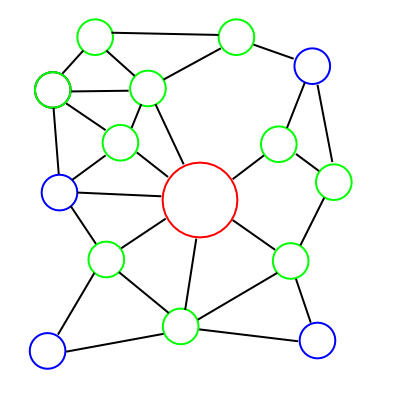
\includegraphics[width=0.4\linewidth]{mesh}
\caption{Schemat topoligii typu mesh.}
\label{fig:Mesh-Network}
\end{figure}

\chapter{Architektura systemu}
\section{Rozmieszczenie komponentów systemu}
Wszystkie komponenty systemu zostały rozmieszczone w taki sposób, aby możliwa była komunikacja pomiędzy poszczególnymi elementami systemu. Aplikacja odpowiedzialna za komunikację z sensorami i elementami aktywnymi, aplikacja internetowa oraz baza danych umieszczone zostały na jednostce bazowej systemu inteligentnego domu.

Rozdzielenie wszystkich komponentów systemu naturalnie wymusiło w projekcie zastosowanie architektury 3-warstwowej:
\begin{enumerate}
	\item \textbf{warstwa prezentacji} – odpowiedzialna za prezentowanie odpowiednio przetworzonych danych użytkownikowi,
	\item \textbf{warstwa biznesowa} – na tym poziomie realizowane są wszystkie operacje biznesowe odpowiedzialne za przetwarzanie danych otrzymanych od użytkownika przed zapisaniem ich do bazy danych lub danych otrzymanych z bazy danych w celu przygotowania ich do ,,pokazania'' użytkownikowi. Są tu również przetwarzane dane przychodzące z czujników oraz wychodzące do elementów aktywnych,
	\item \textbf{warstwa dostępu do danych} – tutaj znajduje się baza danych systemu inteligentnego domu; na tym poziomie dane przechowywane są w sposób ,,zrozumiały'' dla bazy danych.
\end{enumerate}
Rozmieszczenie komponentów systemu w danych warstwach przedstawia poniższy diagram rozmieszczenia:
\clearpage
\begin{figure}[h]
\centering
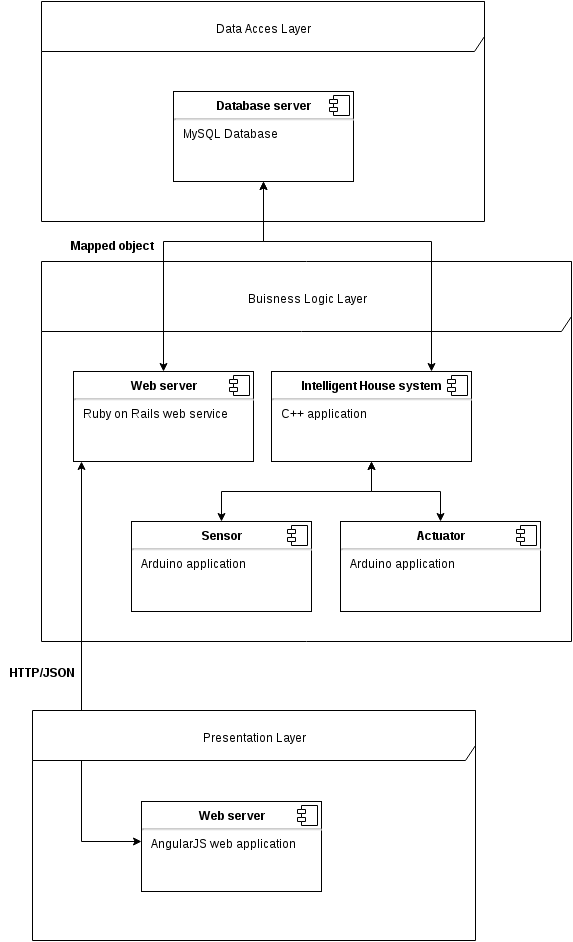
\includegraphics[width=\linewidth]{layers}
\caption{Diagram rozmieszczenia komponentów systemu.}
\label{fig:diagram_rozmieszczenia}
\end{figure}
\clearpage

\section{Diagram klas} % (fold)
\label{sec:diagram_klas}
Poprzez analizę wymagań systemu oraz przypadków użycia, powstał następujący diagram klas, który równocześnie jest odzwierciedleniem schematu bazy danych.
\begin{figure}[h]
\centering
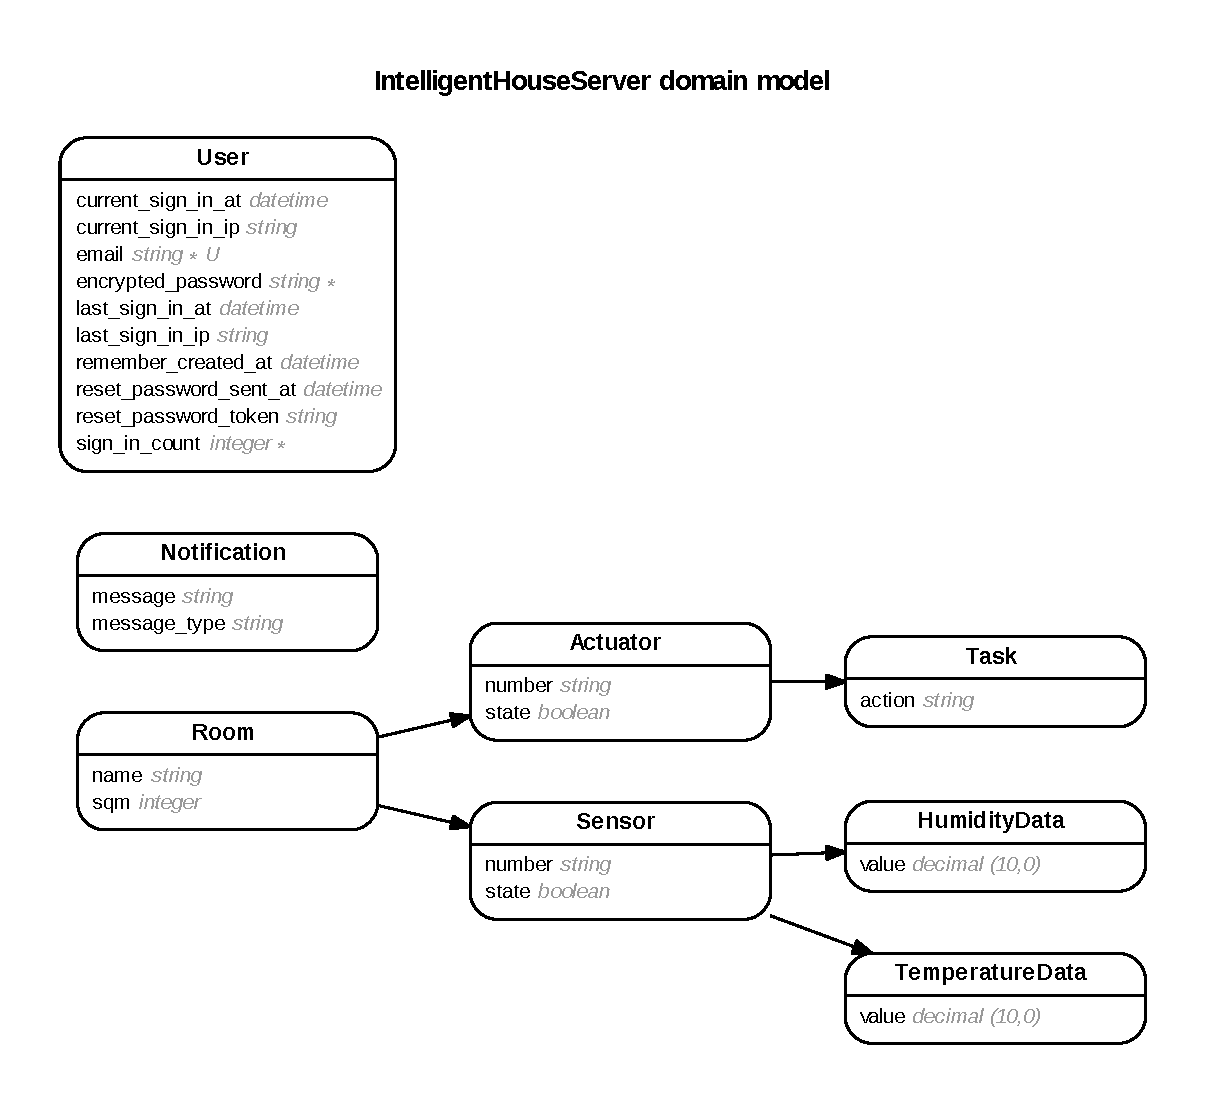
\includegraphics[width=\linewidth]{./erd}
\caption{Diagram klas systemu.}
\label{fig:diagram_encje}
\end{figure}

\section{Topologia systemu inteligentnego domu}
\label{sec:topologia_systemu}
Znaczna większość systemów inteligentnych domów opiera się na topologii gwiazdy. ,,Ramionami'' gwiazdy są sensory i elementy aktywne, natomiast elementem łączącym te ramiona jest system zarządzania. Zastosowanie takiej topologii ma bardzo dużą zaletę - jeśli któryś z sensorów bądź elementów aktywnych przestanie działać, to nie ma to wpływu na działanie pozostałych elementów systemu. Ponadto, dzięki zastosowaniu topologii gwiazdy, system jest bardziej wydajny. Elementy peryferyjne mają ograniczoną moc obliczeniową, a przez to ograniczoną ilość zadań, które mogą wykonać. Większa ilość zadań spoczywających na nich, wymusiłaby zwiększenie mocy obliczeniowej, co automatycznie zwiększyłoby również koszt systemu, a jest to wysoce nieporządane zjawisko. Zamiast tego część zadań należy przydzielić jednostce bazowej, która powinna być najbardziej wydajnym elementem system.


Niestety, z topologią gwiazdy wiąże się spore niebezpieczeństwo, ponieważ jeśli to jednostka bazowa ulegnie awarii, to przestaje działać cały system. 

\begin{figure}[h]
\centering
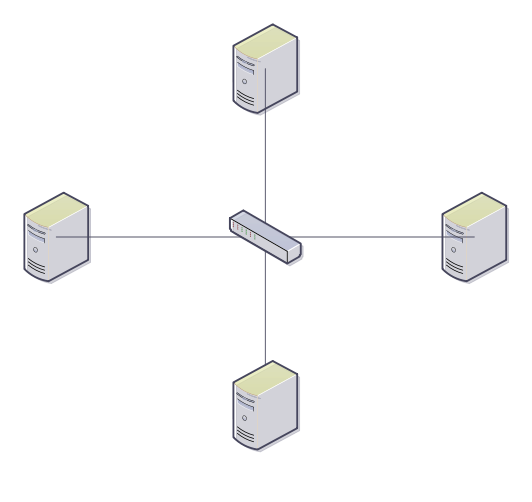
\includegraphics[width=0.6\linewidth]{topologia_gwiazdy}
\caption{Schemat topologii gwiazdy.}
\label{fig:star-network}
\end{figure}

\section{Komunikacja pomiędzy elementami systemu} % (fold)
\label{sec:komunikacja_pomi_dzy_elementami_systemu}
Interfejs komunikacji z elementami inteligentnego domu, aplikacja internetowa oraz baza danych umieszczone są na tym samym serwerze. Całość buduje system zarządzania inteligentnym domem.

Komunikacja pomiędzy elementami inteligentnego domu jest komunikacją bezprzewodową, działającą w topologii opisanej w punkcie \ref{sec:topologia_systemu}. Dane pobrane z sensorów zapisywane są, po odrzuceniu błędów grubych, bezpośrednio do bazy danych. Zmiana stanu elementu aktywnego następuje po pojawieniu się odpowiedniego wpisu w bazie danych w tabeli przechowującej zadania. Jak widać, komunikacja w tej części systemu opiera się na bezprzewodowych technologiach sieciowych oraz na bazie danych.

Back-end aplikacji internetowej jest usługą sieciową zrealizowaną w stylu architektury oprogramowania typu REST, która udostępnia interfejsy komunikacyjne dla warstwy prezentacji aplikacji webowej oraz innych aplikacji, np. aplikacji mobilnej na platformę Android, przy pomocy formatu JSON.

Przykładowe zapytanie zwracające podstawowe dane na temat systemu ma następujący przebieg:
\begin{enumerate}
	\item klient webowy wykonuje zapytanie HTTP GET na adres /dashboard.json,
	\item serwer odbiera zapytanie i na tej podstawie wywołuje funkcję odpowiedzialną za pobranie z bazy danych oraz przetworzenie tych danych, 
	\item rezultat wywołanej funkcji zapisywany jest w formacie JSON i odesłany jako odpowiedź.
\end{enumerate}

Główną zaletą podejścia RESTowego jest ogromna skalowalność aplikacji oraz, w pewnym sensie, jej niezależność. Skalowalność aplikacji polega na tym, że system może być w łatwy sposób rozbudowany, niezależność zaś oznacza, że dla klienta serwer jest czarną skrzynką, do której jest podłączony. W trakcie jego działania możliwa jest zmiana algorytmu przetwarzania danych, bądź też całego back-endu, a mimo wszystko dopóki dane wejściowe i wyjściowe będą takie same – nie odczuje on różnicy. Dodatkowo, gdy wystawiona jest jedna wersja API, można równolegle pracować nad drugą, przykładowo: API v1 wystawione jest dla użytkowników aplikacji klienckiej w wersji $<2.0$, natomiast API v2 obsługuje aplikacje w wersji $\ge2.0$. Dzięki temu możliwy jest rozwój aplikacji z jednoczesnym wsparciem wersji poprzednich. 
% section komunikacja_pomi_dzy_elementami_systemu (end)

\chapter{Specyfikacja systemu}
\section{Aplikacja inteligentnego domu} % (fold)
\label{sec:specyfikacja_aplikacja_inteligentnego_domu}
Aplikacja inteligentnego domu jest odpowiedzialna za komunikację z czujnikami i elementami aktywnymi oraz bazą danych. Jest ona \emph{de facto} interfejsem do komunikacji pomiędzy elementami inteligentnego domu, nie posiada algorytmów sterowania, które znajdują się w webowej części serwera.
Aplikacja ta musi być napisana w języku wspierającym obsługę GPIO (\emph{ang. General Purpose Input Output}) znajdującym się na Raspberry Pi. Językami, które posiadają odpowiednie biblioteki są C++ oraz Python.
% section  (end)

\section{API serwera}
Serwer powinien być rozumiany jako główny element logiki biznesowej systemu. Jest on elementem, który z zewnątrz jest czarną skrzynką, z której korzystają klienci aplikacji webowej. Komunikuje się on z innymi systemami w sposób opisany w punkcie \ref{sec:komunikacja_pomi_dzy_elementami_systemu}.

Poza komunikacją z systemami zewnętrznymi, serwer komunikuje się przede wszystkim bezpośrednio z bazą danych. Jest on miejscem, w którym przeprowadzane są wszystkie operacje pobierania, modyfikowania oraz zapisywania danych do bazy. Przed zapisem bądź po pobraniu danych z bazy są one odpowiednio przetwarzane. Aby zachować poprawność danych, niektóre pola muszą mieć walidację. Jest to realizowane na poziomie bazy danych - przykładowo, jeśli pole, które nie może być puste ma wartość \emph{null}, to baza danych nie pozwoli nam na zapis.

\section{Aplikacja internetowa}
Jako aplikacje internetową należy rozumieć część aplikacji webowej nazywaną ,,front-end’em'', czyli części służącej do komunikacji z użytkownikiem,przez przeglądarkę internetową.

Aplikacja internetowa powinna być wykonana w technologii SPA (\emph{ang. Single Page Application}). Jest to technologia, w której wszystkie elementy strony internetowej, czyli HTML, CSS i JavaScript są pobierane dynamicznie i dołączane do aktualnie wyświetlanej strony w razie potrzeby, najczęsciej po określonych akcjach użytkownika. Strona nie przeładowuje się na żadnym etapie, ponieważ wykorzystuje serwisy do wysłania zapytań do API serwera. Serwisy są asynchroniczne i wykonują się w osobnym wątku. Dzięki takiemu rozwiązaniu użytkownik ma wrażenie ze strona ładuje się natychmiastowo, ponieważ widać jej część, a tak naprawdę większość komponentów czeka na dane zwrócone z API serwera. Przykładowo, po zalogowaniu do aplikacji wykorzystywana jest maszyna stanów adresów, dzięki czemu możliwe jest ładowanie tylko części strony pod paskiem nawigacyjnym, a pasek nawigacyjny zawiera przyciski ładujące odpowiedni widok.

Zastosowaniu takiego rozwiązania przenosi prawie całość obliczeń odpowiedzialnych za wyświetlanie widoków na przeglądarkę internetową, czyli stronę użytkownika. Dzięki temu można odciążyć serwer w przypadku, kiedy nie należy on do najwydajniejszych. W efekcie dane są dostarczane szybko, ich wyświetlanie jest płynne i użytkownik nie musi czekać na przeładowanie strony.

Frameworkami JavaScriptu, które realizują założenia SPA, są AngularJS, Ember.js oraz Meteor.js.

\chapter{Wybrane technologie}
\section{Hardware}
Pod względem sprzętowym, system inteligentnego domu można podzielić na dwie części: elementy peryferyjne oraz jednostkę bazową. Każda z tych części cechuje się innymi wymaganiami odnośnie mocy obliczeniowej, dostępnej pamięci, rozmiarów bądź poboru prądu. Z tego powodu w projekcie zostały wykorzystane dwie platformy - Arduino oraz Raspberry Pi.
\subsection{Sensory i elementy sterujące} % (fold)
\label{sub:sensory_i_elementy_sterujace}
Elementy peryferyjne inteligentnego domu mają kilka głównych wymagań:
\begin{itemize}
	\item nieduża moc obliczeniowa,
	\item niewielki rozmiar,
	\item małe zapotrzebowanie na prąd,
	\item niska cena.
\end{itemize}
W wyniku analizy owych wymagań oraz przeglądu dostępnych rozwiązań, do realizacji czujników i elementów aktywnych zdecydowano się wykorzystać urządznie Arduino Pro Mini 3.3V.

Urządzenie to jest oparte na mikrokontrolerze ATmega328 i działa pod napięciem 3.3V. Zegar taktowany jest z szybkością 8MHz. Mikrokontroler ten posiada 32kB pamięci flash, 2kB pamięci SRAM oraz 1kB pamięci EEPROM. Jego wymiary to 17.7mm x 33mm, więc jest wystarczająco małym urządzeniem. Niewielka wydajność oraz zasilanie napięciem 3.3V skutkuje małym zapotrzebowaniem na prąd. Całość parametrów przekłada się również na cenę - obecnie Arduino Pro Mini można kupić już za 10zł.
% subsection sensory_i_elementy_sterujace (end)

\subsection{Jednostka bazowa} % (fold)
\label{sub:jednostka_bazowa}
Jednostka bazowa powinna nie posiada tylu wymagań, co urządzenia peryferyjne. Nie będzie ona zasilana bateriami, więc zużycie prądu nie gra tu większej roli. Jednostka bazowa jest tylko jedna, więc  rozmiar jest w tym przypadku zależny wymogiem jedynie estetycznym. Jako, że projekt ma być dostępny dla większej ilości ludzi, kwestia ceny ma tutaj sporą rolę i oczywiście komputer zarządzający naszym systemem nie powinien być drogi. Wobec jednostki bazowej jest jedno podstawowe wymaganie - odpowiednia wydajność. Oczywiście, wydajność ta musi być dostosowana do rozmiarów systemu.

Urządzeniami, które najbardziej nadają się do pełnienia roli jednostki bazowej są mikrokomputery. Przykładowymi rozwiązaniami są Raspberry Pi oraz jego klony, czyli Banana Pi i Orange Pi. Różnią się one od siebie przede wszystkim parametrami wydajnościowymi. Każdy z nich ma jednak wystarczającą wydajność do pełnienia roli jednostki bazowej. Jako, że urządzenie Raspberry Pi ma największe wsparcie społeczności, co jest ważnym elementem przy realizacji tego typu projektu, zostało ono wybrane do realizacji funkcji jednostki bazowej systemu inteligentnego domu.

Raspberry Pi w wersji 2 ma następujące parametry:
\begin{itemize}
	\item Procesor czterordzeniowy ARM Cortex-A7, taktowany zegarem o częstotliwości 900 MHz,
	\item 1GB pamięci RAM (wspóldzielonej z GPU),
	\item 40 portów GPIO,
	\item 4 porty USB 2.0,
	\item port Ethernet 10/100,
	\item system operacyjny Windows 10 IoT, Debian GNU/Linux, Fedora, Arch Linux lub FreeBSD.
\end{itemize}

Średnia cena Raspberry Pi 2 wynosi 175zł. Dodatkowo, potrzebny jest zasilacz oraz karta MicroSD, co nieco zwiększa koszt całego urządzenia, lecz nie powinien przekroczyć on 200zł.
% subsection jednostka_bazowa (end)

\section{Software}
\subsection{Aplikacja internetowa}
Serwis internetowy wykonany został w oparciu o następujące technologie:
\begin{itemize}
	\item \textbf{Ruby on Rails} - wnętrze (back-end) portalu webowego, które odpowiedzialne jest za wykonywanie określonych zadań na podstawie danych otrzymanych z fasady (front-end),
	\item \textbf{AngularJS} - fasada (front-end) - jej zadaniem jest komunikacja z użytkownikiem (odbieranie od niego danych oraz przekazywanie ich do back-end'u). AngularJS jest frameworkiem JavaScript'owym, który wymaga stosowania wzorca projektowego \emph{MVC} (ang. Model-View-Controller).
\end{itemize}
Ponadto wykorzystane zostały następujące elementy:
\begin{itemize}
	\item \textbf{CoffeeScript} - język programowania kompilowany do JavaScriptu. Ponieważ CoffeeScript kompiluje się do JavaScriptu, programy mogą być krótsze o około $\frac{1}{3}$ bez strat dla szybkości działania,
	\item \textbf{Slim} – język oparty na szablonach (ang. template language), którego celem jest maksymalna redukcja składni HTML’owej poprzez usunięcie np. tagów zamykających. W efekcie otrzymujemy bardzo czytelny kod, oparty na wcięciach.
\end{itemize}

\subsection{Aplikacja inteligentnego domu} % (fold)
\label{sub:aplikacja_inteligentnego_domu}

% subsection aplikacja_serwerowa (end)

\subsection{Baza danych}
Jako system bazodanowy wykorzystany został MySQL w wersji 5.6. Niewątpliwymi zaletami tego systemu jest to, że posiada on wysoki stopień niezawodności, jest darmowy oraz powszechnie dostępny i wspierany.


\chapter{Implementacja} % (fold)
\label{cha:implementacja}
\section{Back-end} % (fold)
\label{sec:back_end}
Backend aplikacji internetowej jest reprezentowany przez \emph{Model} i~\emph{Controller} we wzorcu \emph{Model-View-Controller}. Aby aplikacja była napisana zgodnie z~dobrymi praktykami programowania, część logiki znajdującej się w~modelach i~kontrolerach, która nie ma cech ww., zostaje przeniesiona do serwisów. Wszystkie kluczowe fragmenty kodu zostaną przedstawione w~kolejnych sekcjach.
\subsection{Modele} % (fold)
\label{sub:modele}
Na obecnym etapie rozwoju aplikacji w~modelach nie ma żadnej dodatkowej logiki. Są tam jedynie opisane relacje z~innymi modelami. Framework \emph{Rails} odpowiednio interreture te informacje, aby pobierać odpowiednie relacje podczas operacji na modelach. Przykładowy model pokazany jest na listingu \ref{lst:sensor}.
\begin{lstlisting}[caption={Model sensora.},label=lst:sensor]
class Sensor < ActiveRecord::Base
  belongs_to :room
end
\end{lstlisting}
Jak widać na powyższym listingu, \emph{Sensor} \textbf{należy do} \emph{Pokoju}.
% subsection modele (end)
\subsection{Logowanie} % (fold)
\label{sub:logowanie}
Logowanie w~aplikacji pełni rolę autentykacji użytkownika. Po zalogowaniu ma on pełny dostęp do wszystkich funkcjonalności systemu. Ponadtko, użytkownik nie jest w~relacji z~żadną inną tabelą. Proces rejestracji i~logowania jest obsługiwany przez dodatek (\emph{gem}) Devise. Jeśli użytkownik nie jest zalogowany, to automatycznie zostaje przekierowany na stronę logowania, gdzie może również zarejestrować nowe konto. Jeśli natomiast przeglądarka zapamiętała sesję, to dostęp do aplikacji nie wymaga ponownego logowania.
% subsection logowanie (end)
\subsection{Pokoje i~sensory} % (fold)
\label{sub:pokoje_i_sensory}
Aby system działał poprawnie, musimy do niego dodać elementy, które zbierają dane. API serwera umożliwia takie akcje poprzez \emph{RoomsController} oraz \emph{SensorsController}. Oba kontrolery są zgodne ze standardem \emph{CRUD} (ang. \emph{Create-Read-Update-Delete}). Dzięki temu Rails'y automatycznie mapują adres na akcję w~kontrolerze. Na listingu \ref{lst:rooms} przedstawiona jest klasa \emph{RoomsController} razem z~odnośnikami oraz rodzajem zapytania HTTP, które prowadzi do danej akcji. Klasa \emph{SensorsController} wygląda analogicznie.
\begin{lstlisting}[caption={RoomsController.},label=lst:rooms]
class RoomsController < ApplicationController
  before_action :set_room, only: [:show, :edit, :update, :destroy]

  # GET /rooms
  # GET /rooms.json
  def index
    render json: Room.all
  end

  # GET /rooms/1
  # GET /rooms/1.json
  def show
  end

  # GET /rooms/new
  def new
    @room = Room.new
  end

  # GET /rooms/1/edit
  def edit
  end

  # POST /rooms
  # POST /rooms.json
  def create
    @room = Room.new(room_params)

    respond_to do |format|
      if @room.save
        format.html { redirect_to @room, notice: 'Room was successfully created.' }
        format.json { render :show, status: :created, location: @room }
      else
        format.html { render :new }
        format.json { render json: @room.errors, status: :unprocessable_entity }
      end
    end
  end

  # PATCH/PUT /rooms/1
  # PATCH/PUT /rooms/1.json
  def update
    respond_to do |format|
      if @room.update(room_params)
        format.html { redirect_to @room, notice: 'Room was successfully updated.' }
        format.json { render :show, status: :ok, location: @room }
      else
        format.html { render :edit }
        format.json { render json: @room.errors, status: :unprocessable_entity }
      end
    end
  end

  # DELETE /rooms/1
  # DELETE /rooms/1.json
  def destroy
    @room.destroy
    respond_to do |format|
      format.html { redirect_to rooms_url, notice: 'Room was successfully destroyed.' }
      format.json { head :no_content }
    end
  end

  private

  # Use callbacks to share common setup or constraints between actions.
  def set_room
    @room = Room.find(params[:id])
  end

  # Never trust parameters from the scary internet, only allow the white list through.
  def room_params
    params.permit(:name, :sqm)
  end
end
\end{lstlisting}
% subsection pokoje_i_sensory (end)
\subsection{Dashboard użytkownika} % (fold)
\label{sub:dashboard_uzytkownika}
Dashboard użytkownika jest miejscem, gdzie wyświetlane są najważniejsze informacje. z~jego poziomu możemy zobaczyć średnią temperaturę oraz wilgotność panujące w~mieszkaniu, ilość aktywnych sensorów, ostatnie wydarzenia w~systemie (np. awaria sensora) oraz wykres temperatury dla ostatniej godziny. Dane te są dostarczane przez \emph{HomeController}.
\begin{lstlisting}[caption={Metoda dashboard odpowiedzialna za generowanie danych dla dashboardu.},label=lst:dashboard]
def dashboard
  avg_temp = TemperatureData.last(100).to_a.sum(&:value) / 100.to_f
  avg_humid = HumidityData.last(100).to_a.sum(&:value) / 100.to_f
  sensors = Sensor.where(state: true).count
  res = {
    avg_temp: avg_temp,
    avg_humid: avg_humid,
    sensors: sensors
  }
  render json: res
end  
\end{lstlisting}
% subsection dashboard_uzytkownika (end)

\subsection{Wykresy} % (fold)
\label{sub:wykresy}
Wykorzystanie systemu przewiduje prezentowanie danych na wykresach. Na listingu \ref{lst:chart_temp} przedstawiony jest kod metody kontrolera, który zwraca tablicę z~temperaturami zebranymi przez każdy z~czujników na przestrzeni ostatniej godziny, tablicę wartości czasowych oraz numery sensorów.
\begin{lstlisting}[caption={Metoda odpowiedzialna za generowanie danych dla wykresów.},label=lst:chart_temp]
def temp_chart
  service = ChartDataService.new(Time.zone.now, 'temperature')
  time = service.create_labels
  data = service.retrive_data
  render json: [data, time, Sensor.where(state: true).pluck(:number)]
end
\end{lstlisting}

Jak widać, kontroler ten korzysta z~serwisu \emph{ChartDataService}, który generuje niebędne dane. Serwis ten jest zbudowany w~taki sposób, że typ danych jest dla niego przezroczysty (podajemy go jako parametr), przez co serwis może pobrane dane przetwarzać identycznie dla różnych typów. Na listingu \ref{lst:chart_service} przedstawiona jest klasa odpowiedzialna za pobieranie danych z~bazy danych, przetworzenie ich oraz zwrócenie tablicy z~danymi, które są przekazywane do kontrolera.
\begin{lstlisting}[caption={Klasa ChartDataService.},label=lst:chart_service]
class ChartDataService
  def initialize(time, type)
    @time = Time.new(time.year, time.month, time.day,
                     time.hour, time.min, 0, Time.zone.now.strftime('%:z'))
    @arr_index = 0
    @type = type
  end

  def retrive_data
    data = []
    Sensor.where(state: true).each do |sensor|
      sensor_data = retrive_sensor_type_data(sensor)
      data << get_data_for_each_minute(sensor, sensor_data)
    end
    data
  end

  def retrive_sensor_type_data(sensor)
    if @type == 'temperature'
      return TemperatureData.where(sensor_id: sensor.id,
                                   created_at: (@time - 1.hour..@time))
    elsif @type == 'humidity'
      return HumidityData.where(sensor_id: sensor.id,
                                created_at: (@time - 1.hour..@time))
    end
  end

  def get_data_for_each_minute(sensor, sensor_data)
    data = []
    (0..59).reverse_each do |amount|
      data_minute = get_array_from_minute(amount, sensor_data, sensor, @time)
      if data_minute.present?
        data << (data_minute.sum(&:value) / data_minute.length.to_f).round(2)
      else
        data << []
      end
    end
    data
  end

  def create_labels
    arr = []
    (0..59).reverse_each do |amount|
      arr << (@time - amount.minute).strftime('%R')
    end
    arr
  end

  def get_array_from_minute(amount, arr, sensor, time)
    return if arr.nil? || arr[@arr_index..-1].nil?
    data = []
    arr[@arr_index..-1].each_with_index do |val, index|
      if val.created_at > time - amount.minute
        @arr_index = index
        break
      end
      data << val if val.sensor_id == sensor.id &&
                     val.created_at <= time - amount.minute &&
                     val.created_at > time - amount.minute - 1.minute
    end
    data
  end
end
\end{lstlisting}
% subsection wykresy (end)
\subsection{Zadania wykonywane w~tle} % (fold)
\label{sub:zadania_wykonywane_w_tle}
Poza standardowymi akcjami wykonywanymi na rządzanie użytkownika, w~systemie zaimplementowana jest dodatkowa akcja. Jest to zadanie wykonywane okresowo oraz ,,w tle''. Do osiągnięcia takiego rezultatu wykorzystywany jest gem \emph{Clockwork}, który odpowiedzialny jest za okresowe wywoływanie zadań. Samo zadanie natomiast jest stworzone przy pomocy mechanizmu znajdującego się w Ruby on Rails - \emph{ActiveJob}. Wywołanie zadania przedstawione jest na listingu \ref{lst:clockwork}, natomiast metoda wywoływana znajduje się na listingu \ref{lst:sensor_job}.
\begin{lstlisting}[caption={Konfiguracja gemu Clockwork.},label=lst:clockwork]
require 'clockwork'
require './config/boot'
require './config/environment'

module Clockwork
  handler do |job, time|
    puts "Running #{job}, at #{time}"
  end

  every(1.minute, 'check sensor statuses') { CheckSensorStateJob.perform_now }
end
\end{lstlisting}

Job ma za zadanie sprawdzać, czy w~ciągu ostatnich 5 minut sensor zarejestrował jakąś wartość. Jeśli tak się nie stało, to ustawiany jest jego stan na \emph{false} oraz dodawana jest notyfikacja do osobnej tabeli. Jeśli sensor był nieaktywny, a~ostatni pomiar jest młodszy niż 5 minut, to stan sensora jest aktualizowany i~ponownie dodawana jest notyfikacja o~przywróceniu sensora do działania.

\begin{lstlisting}[caption={Job uaktualniający stan sensora.},label=lst:sensor_job]
class CheckSensorStateJob < ActiveJob::Base
  queue_as :default

  def perform
    Sensor.all.each do |sensor|
      val = TemperatureData.where(sensor_id: sensor.id).last
      if val.created_at < Time.zone.now - 5.minutes && sensor.state == true
        Notification.create(message: "Sensor #{sensor.number} not responding",
                            message_type: 'error')
        sensor.update_attributes(state: false)
      elsif val.created_at > Time.zone.now - 5.minutes && sensor.state == false
        Notification.create(message: "Sensor #{sensor.number} responding",
                            message_type: 'info')
        sensor.update_attributes(state: true)
      end
    end
  end
end
\end{lstlisting}
% subsection zadania_wykonywane_w_tle (end)
% section back_end (end)
\section{Front-end} % (fold)
\label{sec:front_end}
Front-end aplikacji internetowej składa się z~3 najważniejszych elementów: kontrolerów, serwisów i~widoków. Serwisy komunikują się z~backend'em i~przekazują dane do kontrolerów, które te dane przetwarzają i~przekazują do widoków.
\subsection{Logowanie} % (fold)
\label{sub:logowanie}
Aby po stronie front-endu sprawdzić, czy użytkownik jest zalogowany, pierwszą akcją kontrolera jest wysłanie odpowiedniego zapytania do backendu. Jeśli odpowiedź jest poprawna, to użytkownik może korzystać z zasobów serwisu, natomiast jeśli otrzymana odpowiedź ma status HTTP 401 Unauthorized, to wymagane jest zalogowanie użytkownika. w~takiej sytuacji jest on automatycznie przekierowywany na stronę logowania.
\begin{lstlisting}[caption={Sprawdzenie czy użytkownik jest zalogowany.}, label=lst:front_login]
Auth.currentUser().then((user) ->
      # User was logged in, or Devise returned
      # previously authenticated session.
      $scope.user = user
    (error) ->
      $location.path('/login')
    )
\end{lstlisting}
% subsection logowanie (end)
\subsection{Dashboard} % (fold)
\label{sub:dashboard}
Do pobrania danych wyświetlanych w~dashboardzie użytkownika użyty jest serwis przedstawiony na listingu \ref{lst:dashboard_service}. Serwis ten definiuje metody, które wysyłają zapytanie HTTP GET do aplikacji Railsowej, a~następnie zwraca odebrane dane.
\begin{lstlisting}[caption={Serwis dashboardu.},label=lst:dashboard_service]
angular.module('HouseApp').factory 'Home', ['$http', ($http) ->
  dashboard: () ->
    $http.get('/home/dashboard.json')
  temp_chart: () ->
    $http.get('home/temp_chart.json')
]
\end{lstlisting}

Samo wywołanie metod serwisu odbywa się w~kontrolerze. Zdefiniowane są w nim metody \emph{dashboard(), temp\_chart()} oraz \emph{fetch\_notifications()}, które odpowiedzialne są za wywołanie odpowiednich serwisów i~przypisanie otrzymanych danych do odpowiednich zmiennych znajdujących się w kontrolerze. Fragment kodu kontrolera przedstawiony jest na listingu \ref{lst:dashboard_ctrl}.
\begin{lstlisting}[caption={HomeController.},label=lst:dashboard_ctrl]
angular.module 'HouseApp'
  .controller 'HomeCtrl', ['$http', '$scope', '$location', '$interval', 'Auth', 'Home', 'Notification',
  ($http, $scope, $location, $interval, Auth, Home, Notification)->
  
    $scope.avg = []
    $scope.dashboard = () ->
      Home.dashboard().then((data) ->
        $scope.avg = data.data
      )
    $scope.dashboard()

    $scope.labels = []
    $scope.series = []
    $scope.data = [
      [],
      []
    ]
    $scope.options = {
      pointHitDetectionRadius : 5
    }

    $scope.temp_chart = () ->
      Home.temp_chart().then((data) ->
        $scope.data = data.data[0]
        $scope.labels = data.data[1]
        $scope.series = data.data[2]
      )
    $scope.temp_chart()

    $scope.fetch_notifications = () ->
      Notification.dashboard().then((data) ->
        $scope.notifications = data.data
      )
    $scope.fetch_notifications()
  ]
\end{lstlisting}

Ponadto, dzięki mechanizmowi \emph{two-way binding} znajdującemu się w AngularJS, wyświetlone dane możemy odświeżyć na stronie bez jej przeładowania. Wykorzystując tą cechę, możemy odświeżać dane np. co minutę, co przedstawia listing \ref{lst:interval}
\begin{lstlisting}[caption={Odświeżanie danych co wybrany okres czasu.},label=lst:interval]
$interval (->
  $scope.dashboard()
  $scope.fetch_notifications()
  $scope.temp_chart()
).bind(this), 60000  
\end{lstlisting}
% subsection dashboard (end)
% section front_end (end)
% chapter implementacja (end)

\chapter{Testy} % (fold)
\label{cha:testy}
Aplikacja testowana jest na dwa sposoby: statyczną analizę kodu oraz testy jednostkowe. Narzędziem do statycznej analizy kodu jest Rubocop oraz wtyczka do programu Sublime Text 3, która na bieżąco przeprowadza analizę kodu i~wyświetla znalezione błędy. Testy jednostkowe są przeprowadzane przy pomocy narzędzia RSpec oraz FactoryGirl. 
Wybrałem tą bibliotekę, ponieważ wspiera ona idee Model-View-Controller, w~oparciu o~którą powstała moja aplikacja. Dużą wygodą jest również automatyczna konfiguracja środowiska testowego, która polega m. in.  na osobnej, testowej bazie danych, która jest tworzona na początku wykonywania testów i~czyszczona po zakończeniu każdego przypadku testowege.

RSpec posiada bardzo intuicyjną składnie. Testy podzielone są na 3 poziomową strukturę, każdy poziom zaczyna się słowem kluczowym:
\begin{enumerate}
  \item ,,describe'' – tu definiujemy jaką funkcje/klasę/moduł ma sprawdzać dany zbiór testów,
  \item ,,context'' – to miejsce służy do określenia warunków testu,
  \item ,,it'' – mówi nam jak powinien się zachować testowany moduł.
\end{enumerate}

Przykładowy pojedynczy przypadek testowy:
\begin{lstlisting}[caption={Test kontrolera HomeController.}]
require 'rails_helper'

RSpec.describe HomeController, type: :controller do
  describe 'GET dashboard' do
    before(:each) do
      @sensor = FactoryGirl.create(:sensor)
      @temp = FactoryGirl.create_list(:temperature_data, 60,
                                      sensor_id: @sensor.id)
      t_temp = Time.zone.now
      @t_now = Time.new(t_temp.year, t_temp.month, t_temp.day,
                        t_temp.hour, t_temp.min, 0, Time.zone.now.strftime('%:z'))
      @temp.each_with_index do |temp, index|
        temp.update_attributes(created_at: Time.zone.now - index.minutes)
      end
      @user = FactoryGirl.create(:user)
      sign_in @user
      get :dashboard
    end
    it { is_expected.to respond_with :ok }
    it { expect(response.body.size).to eq(44) }
  end

  describe 'GET temp_chart' do
    before(:each) do
      @sensor = FactoryGirl.create(:sensor)
      @temp = FactoryGirl.create_list(:temperature_data, 60,
                                      sensor_id: @sensor.id)
      t_temp = Time.zone.now
      @t_now = Time.new(t_temp.year, t_temp.month, t_temp.day,
                        t_temp.hour, t_temp.min, 0, Time.zone.now.strftime('%:z'))
      @temp.each_with_index do |temp, index|
        temp.update_attributes(created_at: Time.zone.now - index.minutes)
      end
      @user = FactoryGirl.create(:user)
      sign_in @user
      get :temp_chart
    end
    it { is_expected.to respond_with :ok }
  end
end  
\end{lstlisting}

Powyższy test ma za zadanie sprawdzić czy zapytanie HTTP GET na adresy /dashboard oraz /temp\_chart zostaną przekazane do funkcji ,,dashboard'' oraz ,,temp\_chart'' klasy ,,HomeController'' oraz zwrócą poprawną odpowiedź HTTP ze statusem 200.

Dla ułatwienia wprowadzania atrybutów do testowanych metod lub dodawania rekordów do bazy danych nie wykorzystując napisanych przez siebie metod posłużyłem się biblioteką ,,FactoryGirl'', która implementuje wzorzec projektowy fabryki. Definicja obiektu jest bardzo prosta:

\begin{lstlisting}[language=Ruby, caption={Definicja FactoryGirl.}]
FactoryGirl.define do
  factory :sensor do
    number '123'
    state true
    room
  end
end
\end{lstlisting}
% chapter testy (end)

\chapter{Opis wdrożenia} % (fold)
\label{cha:instrukcja_wdro_enia}
Wdrożenie aplikacji opartej na MySQL, Ruby on Rails oraz AngularJS jest dość prostą czynnością. Na systemie Linux/Unix można ją wykonać w~kilku poniższych krokach:
\begin{enumerate}
  \item instalacja MySQL - najwygodniejsze i~najszybsze jest pobranie bazy danych z~repozytorium,
  \item instalacja ruby - jest kilka narzędzi, które automatyzują proces instalacji Ruby'ego, jednym z~nich jest RVM (\emph{Ruby Version Manager}). Instalacja przebiega w~dwóch krokach (polecenia należy wpisać w~terminalu):
  \begin{enumerate}
    \item gpg --keyserver hkp://keys.gnupg.net --recv-keys 409B6B1796C275462A1703113804BB82D39DC0E3 
    \item \textbackslash{}curl -sSL https://get.rvm.io | bash -s stable
  \end{enumerate}
  \item następnie, w~głównym folderze projektu należy wywołać komendę ,,bundle install'', która zainstaluje wszystkie gemy wymienione w~pliku Gemfile (w tym również framework Rails)
  \item kolejnym krokiem jest utworzenie bazy danych - służy do tego polecenie ,,rake db:create'',
  \item następnie należy wgrać schemat bazy danych oraz ewentualne seedy poleceniem\\,,rake db:migrate db:seed'',
  \item ostatnim etapem jest uruchomienie serwera webowego w~środowisku produkcyjnym bądź developerskim. w~przypadku tego projektu, poza standardowym serwerem znajdującym się w~Railsach, dostępny jest Passenger, którego można uruchomić poleceniem\\,,passenger start -e production'' dla środowiska produkcyjnego,
  \item aby korzstać ze środowiska produkcyjnego, należy przed uruchomieniem serwera webowego wykonać polecenie ,,rake assets:precompile'',
  \item dodatkowo w~programie zaimplementowany jest mechanizm wykonywania zadań w tle o~określonym czasie - aby ta funkcjonalność działała należy uruchomić program clockwork poleceniem ,,clockwork config/clockwork.rb''.
\end{enumerate}
% chapter instrukcja_wdro_enia (end)

\chapter{Instrukcja użytkownika} % (fold)
\label{cha:instrukcja_u_ytkownika}
Pierwszym ekranem, jaki widzi nowy użytkownik, jest ekran rejestracji. z~tego poziomu należy stworzyć konto.
\begin{figure}[h]
\centering
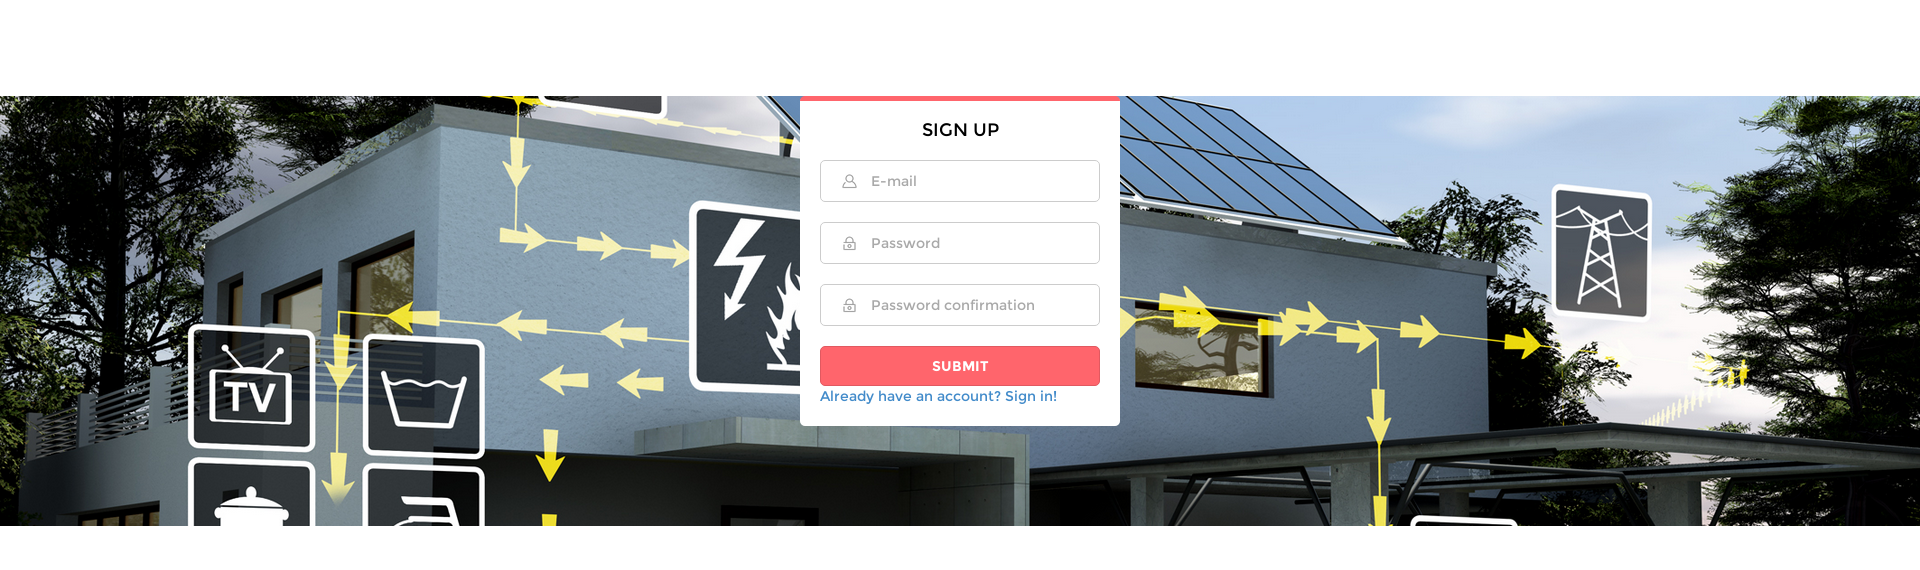
\includegraphics[width=\linewidth]{./register}
\caption{Ekran rejestracji.}
\label{fig:ekran_rejestracji}
\end{figure}

Po założeniu konta użytkownik może zalogować się  do systemu.
\begin{figure}[h]
\centering
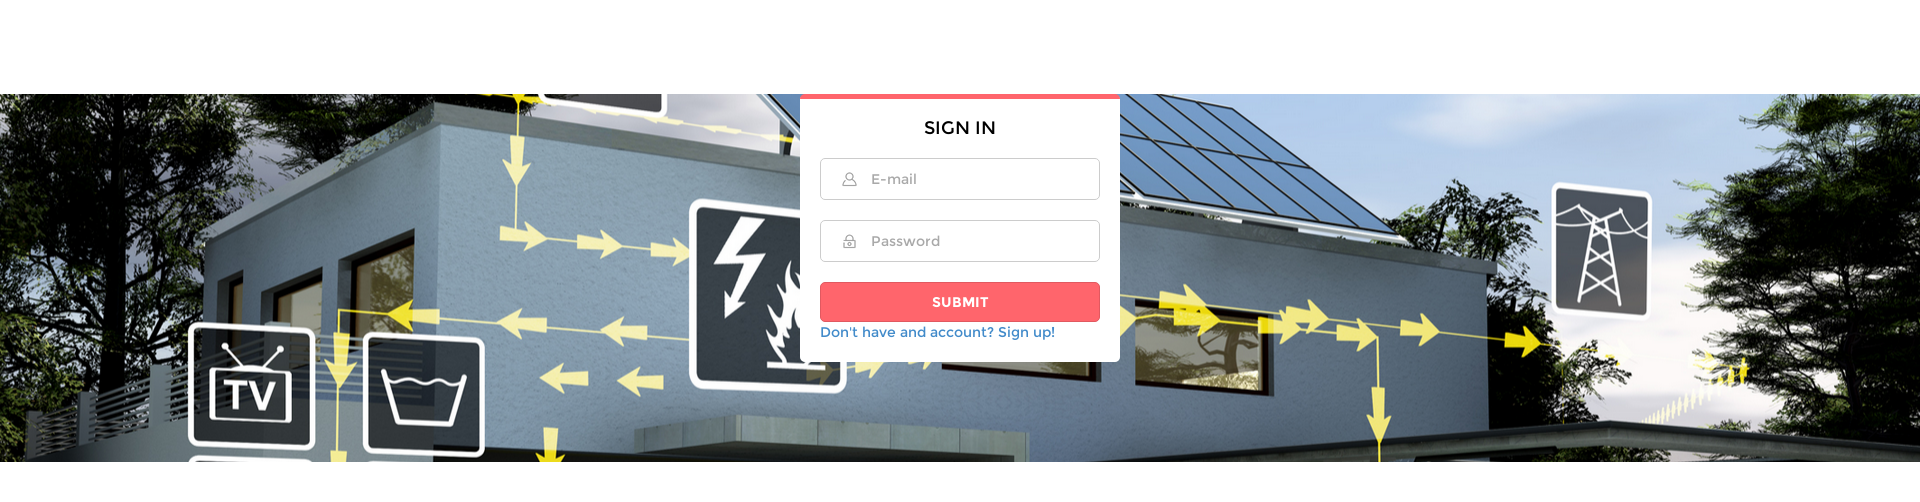
\includegraphics[width=\linewidth]{./login}
\caption{Ekran logowania.}
\label{fig:ekran_logowania}
\end{figure}
% chapter instrukcja_u_ytkownika (end)
\clearpage
Po zalogowaniu użytkownik przekierowywany jest na stronę przedstawiającą dashboard z~najważniejszymi informacjami na temat systemu.
\begin{figure}[h]
\centering
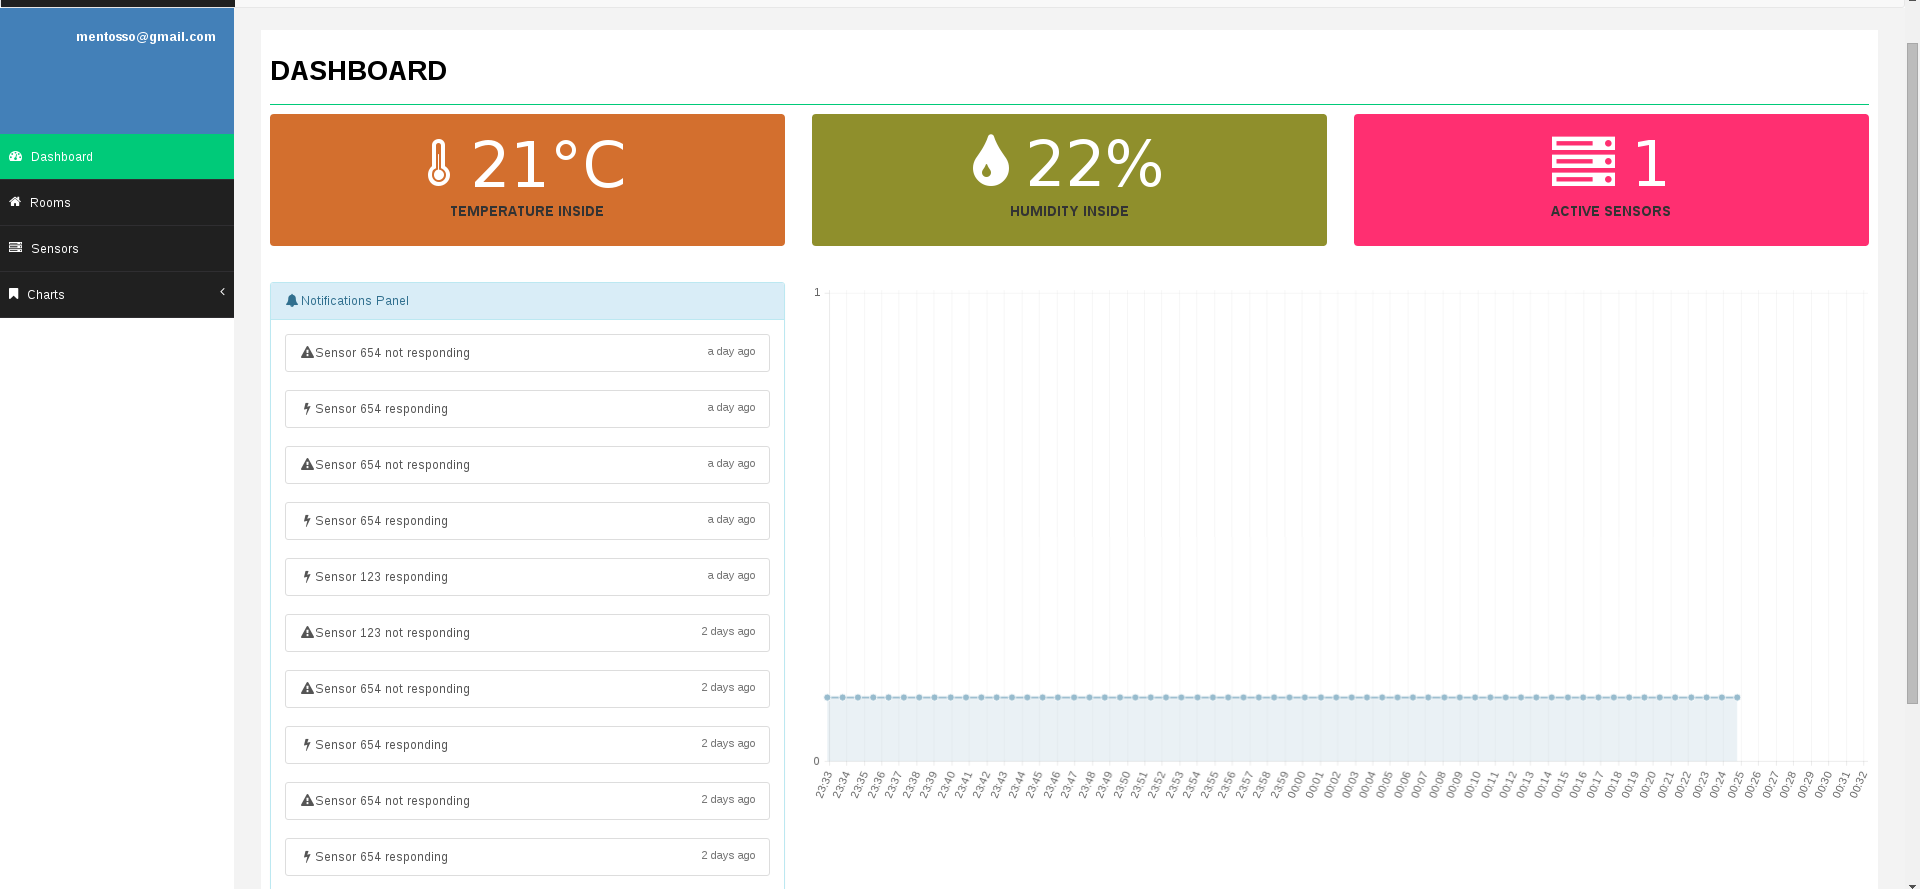
\includegraphics[width=\linewidth]{./dashboard}
\caption{Ekran dashboardu.}
\label{fig:ekran_dashboardu}
\end{figure}

Z poziomu dashboardu użytkownik może dodać nowy pokój, a~następnie dodać do niego sensor.
\begin{figure}[h]
\centering
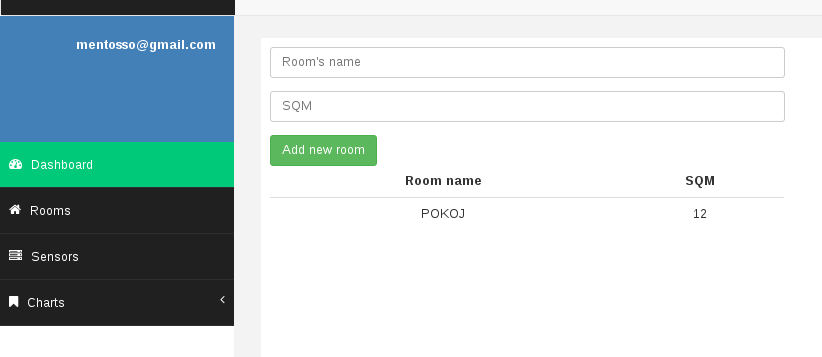
\includegraphics[width=\linewidth]{./rooms1}
\caption{Ekran dodawania pokoi.}
\label{fig:ekran_rejestracji}
\end{figure}
\clearpage
\begin{figure}[h]
\centering
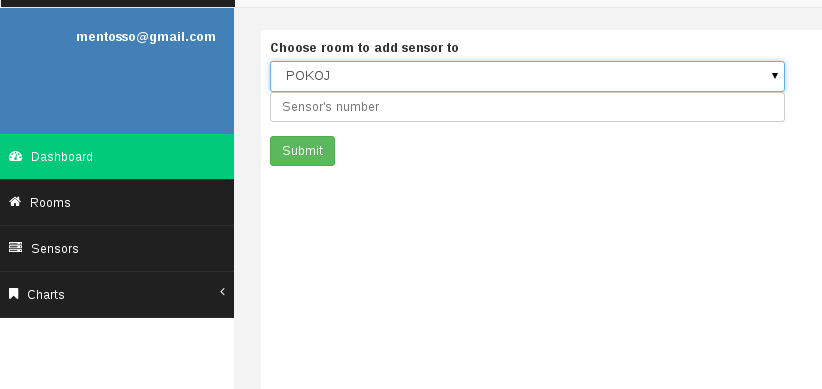
\includegraphics[width=\linewidth]{./sensors}
\caption{Ekran dodawania sensorów.}
\label{fig:ekran_rejestracji}
\end{figure}

Dostępna jest jeszcze zakładka charts, gdzie możemy wybrać ,,Temperature'' oraz ,,Humidity''. Podstrony te prezentują wykresy temperatury lub wilgotności powietrza, takie, jak na stronie dashboardu.

\chapter{Podsumowanie}

\renewcommand\bibname{Literatura}
\begin{thebibliography}{inteligencja}
	\addcontentsline{toc}{chapter}{Literatura}
	
	\bibitem{rails guide}
	\emph{Ruby on Rails Guides}, dostępne pod adresem: \url{http://guides.rubyonrails.org/},\\ aktualne na dzień 14.11.2015r.
	
	\bibitem{angular guide}
	\emph{AngularJS Developer Guide}, dostępne pod adresem: \url{https://docs.angularjs.org/guide}, aktualne na dzień 20.11.2015r.

	\bibitem{arduino}
	\emph{Arduino Pro Mini}, dostępne pod adresem: \url{https://www.arduino.cc/en/Main/ArduinoBoardProMini}, aktualne na dzień 24.11.2015r.

	\bibitem{inteligentne domy}
	Piątek Z., \emph{Od automatyki budynkowej do inteligentnych domów}, dostępne pod adresem \url{http://automatykab2b.pl/}, aktualne na dzień 31.10.2015r.

	\bibitem{magisterka}
	Płachta K., \emph{System komunikacyjny w inteligentnym budynku}, 2012

	\bibitem{cleancode}
	Martin, R. \emph{Czysty kod. Podręcznik dobrego programisty}, Gliwice, Wydawnictwo Helion 2010
	
\end{thebibliography}
\end{document}